\begin{figure}[!tp]
    \centering
    \setlength{\abovecaptionskip}{4pt}
    \setlength{\belowcaptionskip}{-10pt}
    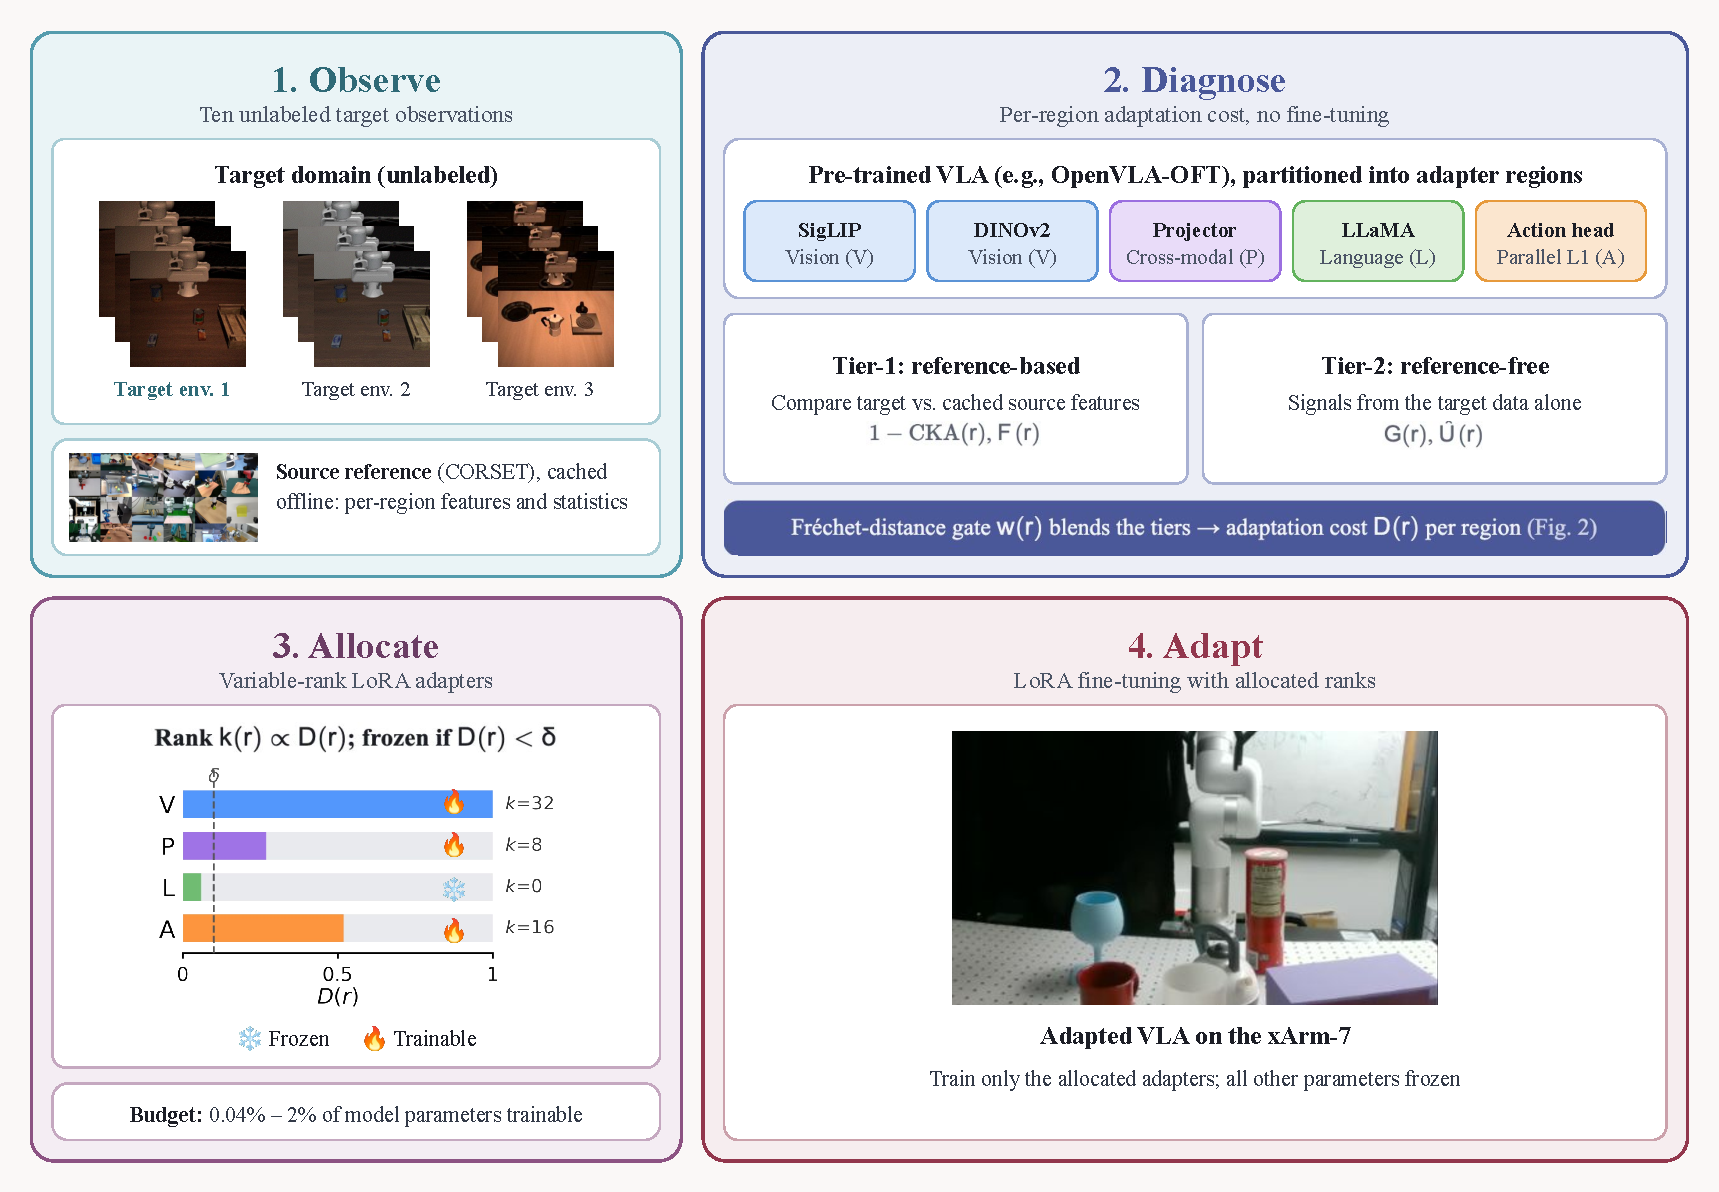
\includegraphics[width=\columnwidth]{images/interpretability_figure1.pdf}
    \caption{\textbf{Observe, diagnose, allocate, adapt.} From a few unlabeled target observations, the pipeline estimates per-region adaptation cost using Tier-1 reference-based signals, Tier-2 reference-free signals, and a Fr\'echet-distance gate to blend them. A budget-aware allocator assigns variable-rank LoRA adapters and freezes well-calibrated regions, and the adapted policy matches full fine-tuning on the xArm-7 at a fraction of the trainable parameters.}
    \label{fig:system-overview}
\end{figure}